\documentclass[11pt]{article}

\usepackage[a4paper,margin=1in]{geometry}
\usepackage{amsmath,amssymb,amsthm,mathtools}
\usepackage{graphicx}
\usepackage{float}
\usepackage{subcaption}
\usepackage{enumitem}
\usepackage{microtype}
\usepackage{xcolor}
\usepackage{hyperref}
\usepackage{fancyhdr}
\usepackage{lastpage}
\usepackage{tikz}
\usetikzlibrary{arrows.meta,calc}

\hypersetup{
  colorlinks=true,
  linkcolor=blue,
  urlcolor=blue,
  citecolor=blue
}

\setlist[enumerate]{itemsep=0.25em,topsep=0.25em}
\setlength{\parindent}{0pt}
\setlength{\parskip}{0.5em}

\theoremstyle{definition}
\newtheorem{exercise}{Exercise}[section]
\newenvironment{solution}{\begin{proof}[Solution]}{\end{proof}}

\DeclareMathOperator{\Area}{Area}
\DeclareMathOperator{\Vol}{Vol}

\newcommand{\HKUSTCrest}{\detokenize{../Week 2/hkust-crest.png}}

\pagestyle{fancy}
\fancyhf{}
\setlength{\headheight}{18.1pt}
\renewcommand{\headrulewidth}{0.4pt}
\fancyhead[L]{\IfFileExists{\HKUSTCrest}{\includegraphics[height=14pt]{\HKUSTCrest}}{}}
\fancyhead[C]{MATH1014 Calculus II Tutorial}
\fancyhead[R]{Week 3}
\fancyfoot[C]{\thepage\ /\ \pageref{LastPage}}

\title{\vspace{-1.0em}MATH1014 Calculus II Tutorial\\Week 3}
\author{Wenkai Fan}
\date{}

\begin{document}
\maketitle
\thispagestyle{fancy}

\section{Review}

\subsection{Volumes}
\begin{enumerate}
  \item Slicing (cross-sectional area / disk or washer method): if the slice area is $A(x)$ for $x\in[a,b]$, then
  \[
  \Vol=\int_a^b A(x)\,dx.
  \]
  \item Cylindrical shells: slice parallel to the axis of rotation.
  \begin{itemize}
    \item Rotating about the $x$-axis (horizontal shells): radius $=y$, height $=x_{\text{right}}(y)-x_{\text{left}}(y)$,
    \[
    \Vol=\int 2\pi\,y\,(x_{\text{right}}(y)-x_{\text{left}}(y))\,dy.
    \]
    \item Rotating about the $y$-axis (vertical shells): radius $=x$, height $=y_{\text{top}}(x)-y_{\text{bottom}}(x)$,
    \[
    \Vol=\int 2\pi\,x\,(y_{\text{top}}(x)-y_{\text{bottom}}(x))\,dx.
    \]
  \end{itemize}
\end{enumerate}

\section{Exercises}

\begin{exercise}[Warm-up: equal volumes]
Find the relationship between $a$ and $c$ such that the volumes generated by rotating the arc segment bounded by $y=x(x-a)$ and $y=0$ around the $x$-axis within the intervals $[0,a]$ and $[a,c]$ are equal.
\end{exercise}

\begin{solution}
\textbf{Step 1: write two volume integrals.} Rotating $y=f(x)$ around the $x$-axis, the disk method gives
\[
\Vol=\int \pi (f(x))^{2}\,dx.
\]
Here $f(x)=x(x-a)$. On $[0,a]$ the curve is below the $x$-axis, but $(f(x))^{2}$ removes the sign. Therefore
\[
V_{1}=\int_{0}^{a}\pi[x(x-a)]^{2}\,dx,\qquad
V_{2}=\int_{a}^{c}\pi[x(x-a)]^{2}\,dx.
\]

\textbf{Step 2: compute and set $V_{1}=V_{2}$.} Expand $[x(x-a)]^{2}=x^{4}-2ax^{3}+a^{2}x^{2}$:
\[
\int \pi[x(x-a)]^{2}\,dx
=\pi\left(\frac{x^{5}}{5}-\frac{a x^{4}}{2}+\frac{a^{2}x^{3}}{3}\right).
\]
So
\[
V_{1}=\pi\cdot\frac{a^{5}}{30},\qquad
V_{2}=\pi\left(\frac{c^{5}}{5}-\frac{a c^{4}}{2}+\frac{a^{2}c^{3}}{3}-\frac{a^{5}}{30}\right).
\]
Setting $V_{1}=V_{2}$ and cancelling $\pi$ gives
\[
2a^{5}+15ac^{4}-10a^{2}c^{3}-6c^{5}=0.
\]
\end{solution}

\begin{exercise}[Shells about the $x$-axis]
Suppose the area of the region enclosed by $y=ax$ ($0<a<1$) and $y=x^2$ is $S_1$ and the area of the region enclosed by these two curves and $x=1$ is $S_2$.
\begin{enumerate}
  \item Choose $a$ such that it minimizes $S_1+S_2$.
  \item Rotate the regions in (1) around the $x$-axis and evaluate the volume.
\end{enumerate}
\end{exercise}

\begin{solution}
\IfFileExists{1.png}{
\begin{figure}[H]
  \centering
  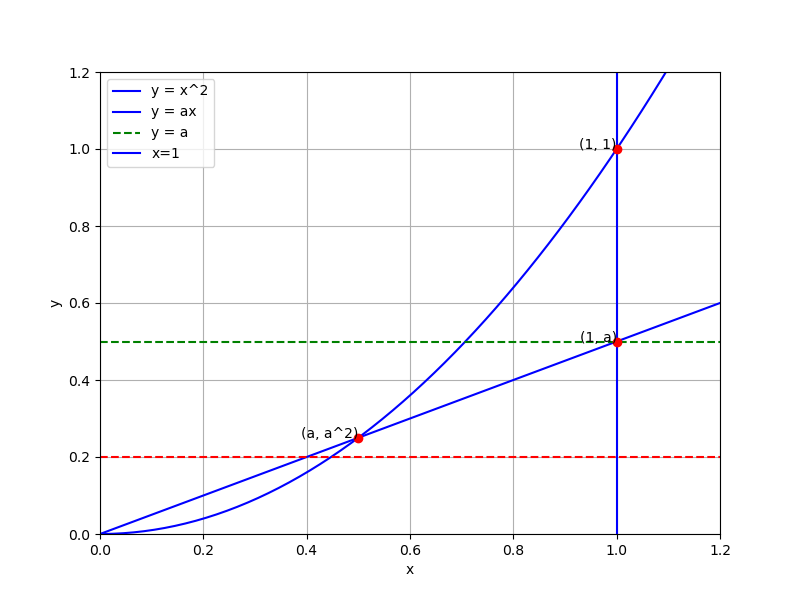
\includegraphics[width=0.75\textwidth]{1}
  \caption*{Geometric picture for Exercise 2.}
\end{figure}
}{}
\textbf{(1) Minimize $S_1+S_2$.} The curves intersect when $ax=x^{2}$, i.e.\ at $x=0$ and $x=a$.
On $[0,a]$, $ax\ge x^{2}$ so
\[
S_1=\int_{0}^{a}(ax-x^{2})\,dx.
\]
On $[a,1]$, $x^{2}\ge ax$ so
\[
S_2=\int_{a}^{1}(x^{2}-ax)\,dx.
\]
Therefore
\begin{align*}
S_1+S_2
&=\int_{0}^{a}(ax-x^{2})\,dx+\int_{a}^{1}(x^{2}-ax)\,dx \\
&=\left.\left(\frac{a x^{2}}{2}-\frac{x^{3}}{3}\right)\right|_{0}^{a}
 +\left.\left(\frac{x^{3}}{3}-\frac{a x^{2}}{2}\right)\right|_{a}^{1} \\
&=\frac{1}{3}a^{3}-\frac{1}{2}a+\frac{1}{3}.
\end{align*}
Let $f(a)=\frac{1}{3}a^{3}-\frac{1}{2}a+\frac{1}{3}$. Then
\[
f'(a)=a^{2}-\frac{1}{2}.
\]
On $(0,1)$ the critical point is $a=\frac{\sqrt{2}}{2}$, and $f''(a)=2a>0$, so it gives the minimum:
\[
a=\frac{\sqrt{2}}{2}.
\]

\textbf{(2) Volume by cylindrical shells (about the $x$-axis).} We use \emph{horizontal} shells at height $y$.
Each shell has radius $y$ and thickness $dy$, and its height is the horizontal length of the region at that $y$.

Because the right boundary $x=1$ is present in $S_2$, the shell height changes depending on $y$:
\begin{enumerate}
  \item For $0\le y\le a^{2}$: the horizontal line meets $y=ax$ at $x=\frac{y}{a}$ and meets $y=x^{2}$ at $x=\sqrt{y}$. In this range, the region from $S_1$ contributes height $\sqrt{y}-\frac{y}{a}$.
  \item For $a^{2}\le y\le a$: the region comes from $S_2$ between the same two curves, so the height is $\frac{y}{a}-\sqrt{y}$.
  \item For $a\le y\le 1$: the line $y=ax$ is above $x=1$ (since $y/a\ge 1$), so the region is between $x=\sqrt{y}$ and $x=1$, hence height $1-\sqrt{y}$.
\end{enumerate}
Thus
\begin{align*}
V
&=\int_{0}^{a^{2}}2\pi y\left(\sqrt{y}-\frac{y}{a}\right)dy
 +\int_{a^{2}}^{a}2\pi y\left(\frac{y}{a}-\sqrt{y}\right)dy
 +\int_{a}^{1}2\pi y(1-\sqrt{y})dy \\
&=2\pi\left[\left.\left(\frac{2}{5}y^{\frac{5}{2}}-\frac{y^{3}}{3a}\right)\right|_{0}^{a^{2}}
 +\left.\left(\frac{y^{3}}{3a}-\frac{2}{5}y^{\frac{5}{2}}\right)\right|_{a^{2}}^{a}
 +\left.\left(\frac{y^{2}}{2}-\frac{2}{5}y^{\frac{5}{2}}\right)\right|_{a}^{1}\right] \\
&=2\pi\left(\frac{2}{15}a^{5}-\frac{1}{6}a^{2}+\frac{1}{10}\right).
\end{align*}
Substitute $a=\frac{\sqrt{2}}{2}$:
\[
V=\frac{\sqrt{2}+1}{30}\pi.
\]
\end{solution}

\end{document}
